% !TEX TS-program = pdflatex
% !TEX encoding = UTF-8 Unicode

\documentclass[12pt,a4paper]{article}
\usepackage{incgraph,microtype,tikz,colortbl,pdflscape,moresize,lmodern,enumitem,wrapfig}

\usepackage[paperwidth=100mm, paperheight=160mm,left=0.5cm,right=0.5cm,top=.5cm,bottom=.5cm,textwidth=5cm,textheight=5cm]{geometry}

\newgeometry{paperwidth=100mm, paperheight=160mm, vmargin={5mm}, hmargin={7mm,17mm}}   % set the margins

\usepackage{relsize}
\usepackage[sfdefault,scaled=1]{FiraSans}

\usepackage{mathrsfs}

\usepackage[utf8]{inputenc}
\usepackage[T1]{fontenc}
\usepackage[main=english,french,german]{babel}

\usepackage{pagecolor}

\pdfminorversion=4

\pagestyle{plain}

\usepackage{setspace}
\setstretch{0.8}

\sloppy

\usepackage{array}

\hypersetup{
    colorlinks,
    linkcolor=, %linkcolor={red!50!black},
    citecolor={blue!50!black},
    urlcolor={blue!80!black}
}

% \newcommand{\person}[4]{~\newline\vspace{-1mm}
% % \begin{minipage}{\textwidth}
% \begin{wrapfigure}[7]{l}{2.15cm}
% \vspace*{-1.3\baselineskip}%
% \centering
% \personphoto{#4}
% \end{wrapfigure}
% \emph{\relscale{0.9}#3}
% % \end{minipage}
% } 

\title{SIGMOD 2019}

\begin{document}

\pagestyle{empty}


%!TEX root = schedule.tex

\tikzset{
  headings/base/.style = {
    outer sep = 0pt,
    text width = {\textwidth - 0.6666em},
    align = center,
    text = white,
    font = \sffamily\Large\bfseries
  },
  headings/slot/.style = {
    headings/base,
    fill = black!90,
    rounded corners=.5mm,
    font = \sffamily\huge\bfseries
  },
  headings/session/.style = {
    headings/base,
    fill = black!70,
    align = center,
    rounded corners=.5mm
    % font = \sffamily\Large\bfseries
  }
}

\hypersetup{
    colorlinks,
    linkcolor=, %linkcolor={red!50!black},
    citecolor={blue!50!black},
    urlcolor= %{blue!80!black}
}

\newcommand{\slotheading}[1]{\newpage

\begin{center}
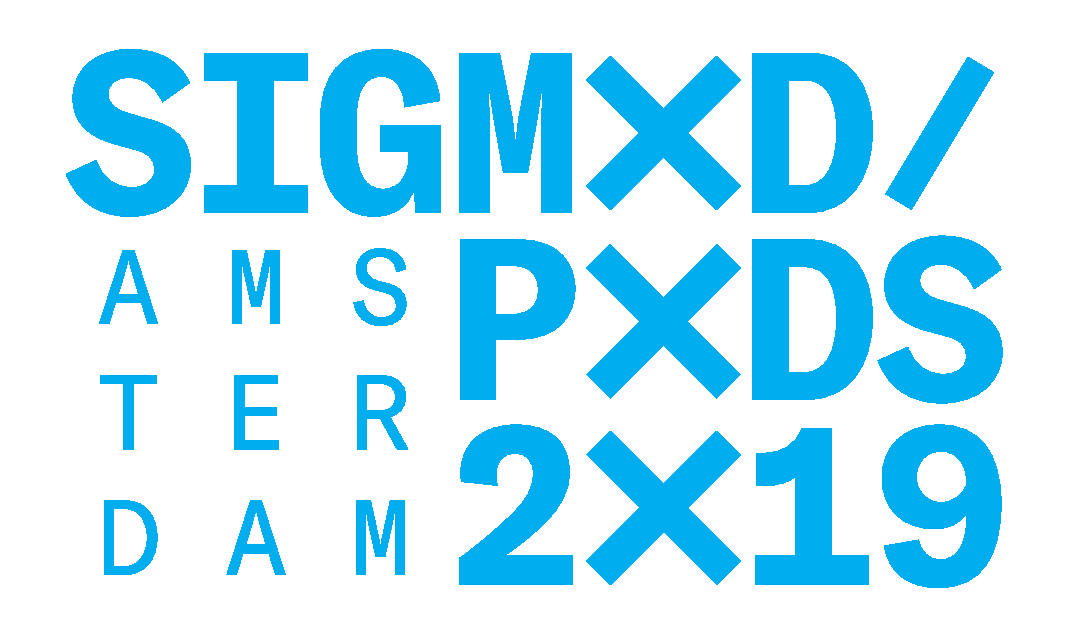
\includegraphics[width=.65\textwidth]{sigmod_logo.pdf}
\end{center}

 \noindent\tikz{\node[headings/slot]{\textbf{#1}};}}

\newcommand{\sessionname}[2]{\large\noindent\hypertarget{#1}{}\tikz{\node[headings/session]{#2};}}
\newcommand{\sessionnamenl}[1]{\large\noindent\tikz{\node[headings/session]{#1};}}
\newcommand{\sessionlocation}[1]{}%\noindent \textbf{Room}: #1
\newcommand{\sessiontimeloc}[2]{\large\noindent \textbf{Room:} #2 \hfill \textbf{Time}: #1} 

\newcommand{\sessionchair}[1]{\large\noindent \textbf{Chair}: #1}
\newcommand{\sessionsep}{\vspace{2mm}}

\newcommand{\papertitle}[2]{\large\noindent\href{#2}{\textbf{#1}}}
\newcommand{\paperauthors}[1]{\large\\{\relscale{0.9}\em #1}\vspace{2mm}}





